\documentclass[11pt]{beamer}
\usepackage{amsmath,amsfonts}	% use math symbols
\usepackage{graphicx} % insert images
\usepackage{url} % insert urls
\usepackage{hyperref}
\hypersetup{
	linkcolor  = blue,
	citecolor  = blue,
	urlcolor   = blue,
	colorlinks = true,
}
\usepackage{amsthm}
%\usepackage{auto-pst-pdf}
\setbeamertemplate{navigation symbols}{}
\usepackage{listings}
\usepackage{xcolor}
\usepackage{moresize}

\definecolor{cream}{rgb}{1.0, 0.99, 0.82}

\lstset{frame=single, basicstyle=\color{black}\ttfamily\tiny, backgroundcolor=\color{cream}}



%%%%%%%%%%%%%%%%%%%%%%%%%%%%%%%%%%%%%%%%%%%%



\begin{document}

\title{Introduction to Git}
\author{Daniel Lin}
\date{}


\maketitle

%%%%%%%%%%%%%%%%%%%%%%%%%%%%%%%%%%%%
\begin{frame}
\frametitle{Outline}
\tableofcontents
\end{frame}

%%%%%%%%%%%%%%%%%%%%%%%%%%%%%%%%%%%%
\section{Introduction}
\begin{frame}{What is version control?}
\begin{itemize}
\item
A system that keeps records of your changes (commit)
	\begin{itemize}
		\item Who
		\item When
		\item What
		\item Why
	\end{itemize}
\item
Allows for collaborative development
\item
Allows you to revert any changes and go back to a previous state.
\item
Notifies conflict between different versions and allows the possibility of merging
\end{itemize}
\end{frame}

%%%%%%%%%%%%%%%%%%%%%%%%%%%%%%%%%%%%
\begin{frame}{What is Git?}
Git is one of many version control systems.
\begin{itemize}
	\item
	Users can keep entire code and history on their location machines
	\begin{itemize}
		\item Can make any changes without internet access
		\item Except pushing and pulling changes from a remote server
	\end{itemize}
	\item
	It is widely used, both because it's easy to set up and the hosting site, GitHub
\end{itemize}
\end{frame}

%%%%%%%%%%%%%%%%%%%%%%%%%%%%%%%%%%%%
\section{Key Concepts}
\begin{frame}{Key Concepts}
\begin{itemize}
	\item
	\hyperlink{snap}{Snapshots}
	\item
	\hyperlink{commit}{Commit}
	\item
	\hyperlink{repo}{Repositories}
	\item
	\hyperlink{push}{Push/Pull}
	\item
	\hyperlink{branch}{Branches}	
\end{itemize}
\end{frame}

%%%%%%%%%%%%%%%%%%%%%%%%%%%%%%%%%%%%
\begin{frame}{Snapshots}\label{snap}
\begin{itemize}
	\item
	The way git keeps track of your code history
	\item
	Record of what all your files look like at a given point in time
	\item
	\textbf{You} decide when to take a snapshot and of what files
	\item
	Have the ability to go back to visit any snapshot
\end{itemize}
\end{frame}

%%%%%%%%%%%%%%%%%%%%%%%%%%%%%%%%%%%%
\begin{frame}{Commit}\label{commit}
\begin{itemize}
	\item
	The act of creating a snapshot
	\item
	Essentially, a project is made up of a bunch of commits
	\item
	\textcolor{blue}{\textbf{Commits}} contain these information
	\begin{itemize}
		\item How the files changed from previous state
		\item A reference to the commit that came before it
		\item Comment from the person who made the commit
		\item A hash code name
		\begin{itemize}
			\item e.g. b05d7611c608d160619ddaae23a5d8b02ee9d1d6
		\end{itemize}
	\end{itemize}
\end{itemize}
\end{frame}

%%%%%%%%%%%%%%%%%%%%%%%%%%%%%%%%%%%%
\begin{frame}{Repositories}\label{repo}
\begin{itemize}
	\item
	A collection of all the files and the history of those files
	\begin{itemize}
		\item Consists of all your commits
		\item Place where all your work is stored		
	\end{itemize}
	\item	
	Can live on a local machine or on a remote server (GitHub, ECCO, CISER)
	\item	
	The act of copying a repository from a remote server is called cloning
	\item	
	Cloning from a remote server allows teams to work together
\end{itemize}
\end{frame}

%%%%%%%%%%%%%%%%%%%%%%%%%%%%%%%%%%%%
\begin{frame}{Push/Pull}\label{push}
\begin{itemize}
	\item 
	\textcolor{blue}{\textbf{Push}}
	\begin{itemize}
		\item
		The process of uploading your local changes to the remote repository
	\end{itemize}
	\item 
	\textcolor{blue}{\textbf{Pull}}
	\begin{itemize}
		\item
		The process of downloading commits that don't exist on your machines from a remote repository
	\end{itemize}
\end{itemize}
\end{frame}

%%%%%%%%%%%%%%%%%%%%%%%%%%%%%%%%%%%%
\begin{frame}{Branches}\label{branch}
\begin{itemize}
	\item
	All commits in git live on some branch
	\item
	The main branch in a project is called the \textcolor{blue}{\textbf{master}} branch
\end{itemize}
\end{frame}

%%%%%%%%%%%%%%%%%%%%%%%%%%%%%%%%%%%%
\begin{frame}{What does a typical project look like?}
\begin{itemize}
	\item
	A bunch of commits linked together that live on some branch, contained in a repository
	\item
	You can make change to the master branch directly
	\item
	Or you can make a new branch pointing to a specific commit in the master branch
	\item
	Once you're done with your changes, you can merge the new branch back into master
\end{itemize}
\end{frame}

%%%%%%%%%%%%%%%%%%%%%%%%%%%%%%%%%%%%
\section{Tutorial}
\begin{frame}[fragile]{Tutorial}

\begin{itemize}
	\item \textcolor{blue}{\emph{git init}}
	\item \textcolor{blue}{\emph{git status}}
	\item \textcolor{blue}{\emph{git add}}
	\item \textcolor{blue}{\emph{git diff}}
	\item \textcolor{blue}{\emph{git commit}}
	\item \textcolor{blue}{\emph{gitignore}}
	\item \textcolor{blue}{\emph{git push}}
	\item \textcolor{blue}{\emph{git pull}}
	\item \textcolor{blue}{\emph{git clone}}
\end{itemize}
\end{frame}

%%%%%%%%%%%%%%%%%%%%%%%%%%%%%%%%%%%%
\begin{frame}[fragile]{Install git and Create GitHub account}
Install git
\begin{itemize}
	\item Windows
	\begin{itemize}
		\item \href{https://git-scm.com/download/win}{https://git-scm.com/download/win}
	\end{itemize}
	\item Mac
	\begin{itemize}
		\item \href{https://git-scm.com/download/mac}{https://git-scm.com/download/mac}
	\end{itemize}
	
	\item Linux
	\begin{itemize}
		\item Command: sudo apt-get install git
	\end{itemize}	
\end{itemize}
Create GitHub account
\begin{itemize}
	\item Go to \href{https://github.com/}{GitHub}
\end{itemize}
\end{frame}

%%%%%%%%%%%%%%%%%%%%%%%%%%%%%%%%%%%%
\begin{frame}[fragile]{Set Up}

For your first time with Git on a new machine
\begin{lstlisting}
$ git config --global user.name "Daniel Lin"
$ git config --global user.email "cdl77@cornell.edu"
$ git config --global color.ui "auto"
$ git config --global core.editor "nano"
\end{lstlisting}

You can check common git commands by typing
\begin{lstlisting}
$ git help
\end{lstlisting}
\end{frame}
%%%%%%%%%%%%%%%%%%%%%%%%%%%%%%%%%%%%
\begin{frame}[fragile]{Create an Online Repository}
\begin{center}
	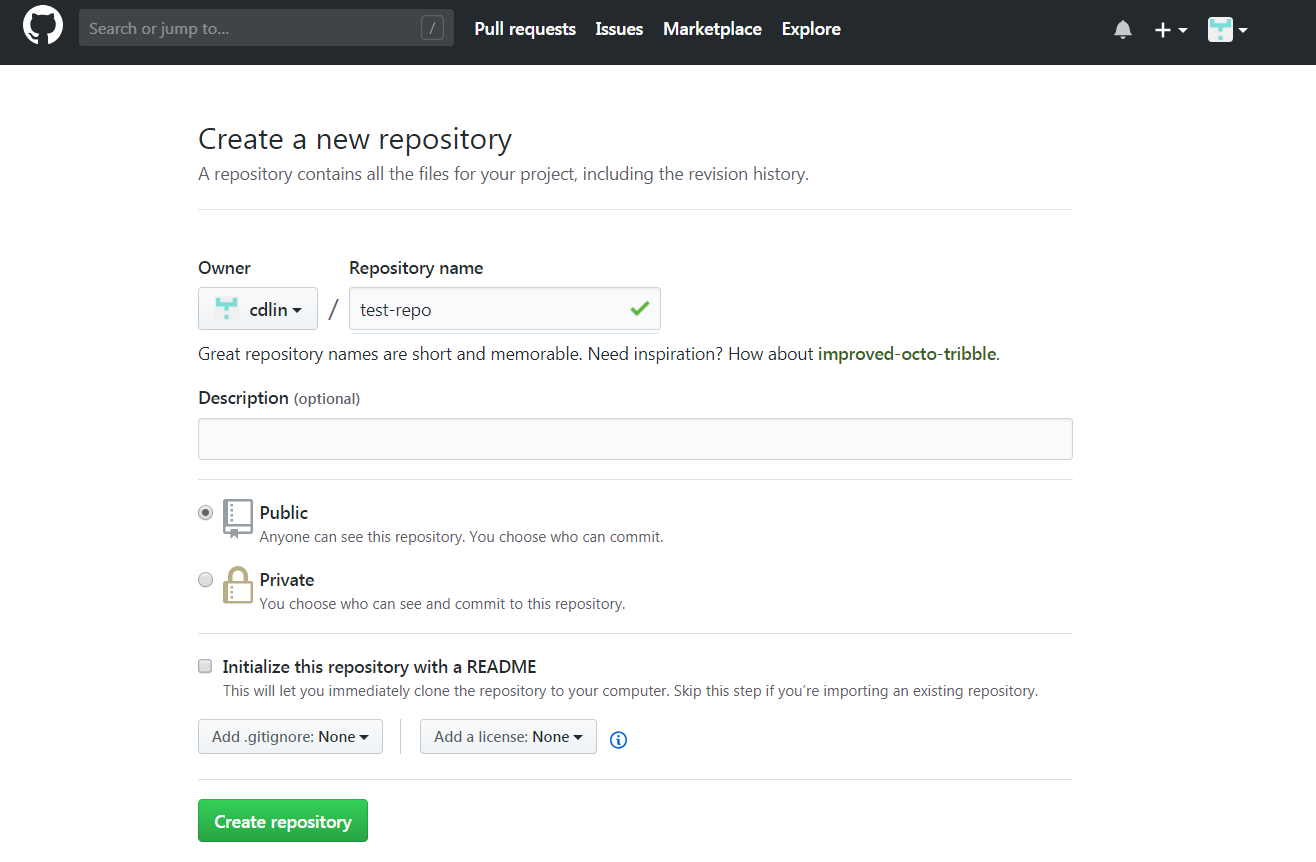
\includegraphics[width=1.0\textwidth]{./auxfiles/github_repo.png}
\end{center}
\end{frame}
%%%%%%%%%%%%%%%%%%%%%%%%%%%%%%%%%%%%
\begin{frame}[fragile]{Create a Local Repository}
Let's create a "myrepo" folder on your desktop and change your directory to it
\begin{lstlisting}
$ cd ~/Desktop
$ mkdir myrepo
$ cd myrepo/
\end{lstlisting}
Use \textcolor{blue}{\emph{git init}} to make it into a \textbf{repository}
\begin{lstlisting}
$ git init
Initialized empty Git repository in
 C:/Users/Daniel/Desktop/myrepo/.git/
\end{lstlisting}
\end{frame}

%%%%%%%%%%%%%%%%%%%%%%%%%%%%%%%%%%%%
\begin{frame}[fragile]{Add New File to Local Repo}
You can use any text editor or run the \textcolor{blue}{\emph{touch}} command
\begin{lstlisting}
$ touch code.do
$ ls
code.do
\end{lstlisting}
You can edit it using the \textcolor{blue}{\emph{nano}} command
\begin{lstlisting}
$ nano code.do
\end{lstlisting}
Type a random sentence
\begin{lstlisting}
This is a test.
\end{lstlisting}
Press CTRL+X to exit, press Y to save the change, press ENTER to confirm the file that is being overwritten
\end{frame}

%%%%%%%%%%%%%%%%%%%%%%%%%%%%%%%%%%%%
\begin{frame}[fragile]{Git Status}

Enter \textcolor{blue}{\emph{git status}}
\begin{lstlisting}
$ git status
On branch master

No commits yet

Untracked files:
	(use "git add <file>..." to include in what will be committed)

		code.do

nothing added to commit but untracked files present (use "git add" to track)
\end{lstlisting}
The output states that we are located on the master branch. The \emph{Untracked files} message means that there are files in the directory that Git is not keeping track of.
\end{frame}
%%%%%%%%%%%%%%%%%%%%%%%%%%%%%%%%%%%%
\begin{frame}[fragile]{Staging Environment}
\begin{itemize}
	\item  A commit is a record of what files you have changed since the last time you made a commit.
 	\item How do you tell git which files to put into a commit?
	\begin{itemize}
		\item Add the files to the Staging Environment using \textcolor{blue}{\emph{git add}}
		\item You can then tell git to package all the files in the staging environment into a commit using the \textcolor{blue}{\emph{git commit}} command
	\end{itemize}
	
\end{itemize}
\end{frame}
%%%%%%%%%%%%%%%%%%%%%%%%%%%%%%%%%%%%
\begin{frame}[fragile]{Git Add}
We tell Git to stage untracked/modified files using \textcolor{blue}{\emph{git add}}
\begin{lstlisting}
$ git add code.do
\end{lstlisting}
and check the status again
\begin{lstlisting}
$ git status
On branch master

No commits yet

Changes to be committed:
  (use "git rm --cached <file>..." to unstage)

	new file:   code.do
\end{lstlisting}

So git knows that it needs to keep track of the file \emph{code.do} but has not yet recorded the changes. 
\end{frame}

%%%%%%%%%%%%%%%%%%%%%%%%%%%%%%%%%%%%
\begin{frame}[fragile]{Git Commit}
Let's \textcolor{blue}{\emph{git commit}} the added changes. 
\begin{lstlisting}
$ git commit -m "First draft code.do"
[master (root-commit) 887d395] First draft code.do
1 file changed, 1 insertion(+)
create mode 100644 code.do
\end{lstlisting}
\begin{itemize}
\item
Git takes everything we have told it to save and stores a copy permanently inside the special .git directory.
\item
This commit has a short identifier 887d395.
\item
 -m flag to record a comment that will help us remember later on what we did and why.
\end{itemize}
Now let's check the status again
\begin{lstlisting}
$ git status
On branch master
nothing to commit, working directory clean
\end{lstlisting}
Everything is up to date and committed.
\end{frame}


%%%%%%%%%%%%%%%%%%%%%%%%%%%%%%%%%%%%
\begin{frame}[fragile]{gitignore}
Sometimes you don't want git to track certain files (large datasets, logs, auxiliary files)
Let's create some files
\begin{lstlisting}
$ touch 2yr_paper.tex
$ touch 2yr_paper.aux
\end{lstlisting}

Git will ignore any changes to anything listed in \textcolor{blue}{\emph{.gitignore}}.
\begin{lstlisting}
$ nano .gitignore
\end{lstlisting}
\begin{lstlisting}
*.aux
*.log
*.gz
\end{lstlisting}
\tiny Press CTRL+X to exit, Y to save, ENTER to confirm

\normalsize 
We have told Git to ignore any file whose name ends in .aux, .log and .gz. 
\end{frame}

%%%%%%%%%%%%%%%%%%%%%%%%%%%%%%%%%%%%
\begin{frame}[fragile]{gitignore}
After we have created the .gitignore file, let's check \textcolor{blue}{\emph{git status}} again
\begin{lstlisting}
$ git status
On branch master
Untracked files:
  (use "git add <file>..." to include in what will be committed)

	.gitignore
	2yr_paper.tex

nothing added to commit but untracked files present (use "git add" to track)
\end{lstlisting}
Git no longer notices the auxiliary latex files.

\end{frame}

%%%%%%%%%%%%%%%%%%%%%%%%%%%%%%%%%%%%
\begin{frame}[fragile]{Modifying files}

Now let's edit our \emph{code.do} file and check the status again.
\begin{lstlisting}
$ nano code.do
\end{lstlisting}
\begin{lstlisting}
This is a test.
Let's add a second line.
\end{lstlisting}
\begin{lstlisting}
$ git status
On branch master
Changes not staged for commit:
  (use "git add <file>..." to update what will be committed)
  (use "git checkout -- <file>..." to discard changes in working directory)

    modified:   code.do

Untracked files:
  (use "git add <file>..." to include in what will be committed)

    .gitignore
    2yr_paper.tex

no changes added to commit (use "git add" and/or "git commit -a")
\end{lstlisting}
As well as the untracked files in the previous status check, Git also tells us that \emph{code.do} has been modified.
\end{frame}

%%%%%%%%%%%%%%%%%%%%%%%%%%%%%%%%%%%%

\begin{frame}[fragile]{Git diff}
Use \textcolor{blue}{\emph{git diff}} to check the change from the previous commit before we add the files
\begin{lstlisting}
$ git diff
diff --git a/code.do b/code.do
index 484ba93..067f664 100644
--- a/code.do
+++ b/code.do
@@ -1 +1,2 @@
This is a test.
+Let's add a second line.
\end{lstlisting}
\end{frame}
%%%%%%%%%%%%%%%%%%%%%%%%%%%%%%%%%%%%
\begin{frame}[fragile]{Complete the Commit}
 Let's now add and commit these changes.
\begin{lstlisting}
$ git add code.do
$ git status
$ git commit -m "New tex file and added line to code.do"
\end{lstlisting}
and checking the status....
\begin{lstlisting}
$ git status
On branch master
nothing to commit, working directory clean
\end{lstlisting}
... we're back to a clean sheet.
\end{frame}

%%%%%%%%%%%%%%%%%%%%%%%%%%%%%%%%%%%%
\begin{frame}[fragile]{Connecting Local and Online Repositories}
\begin{center}
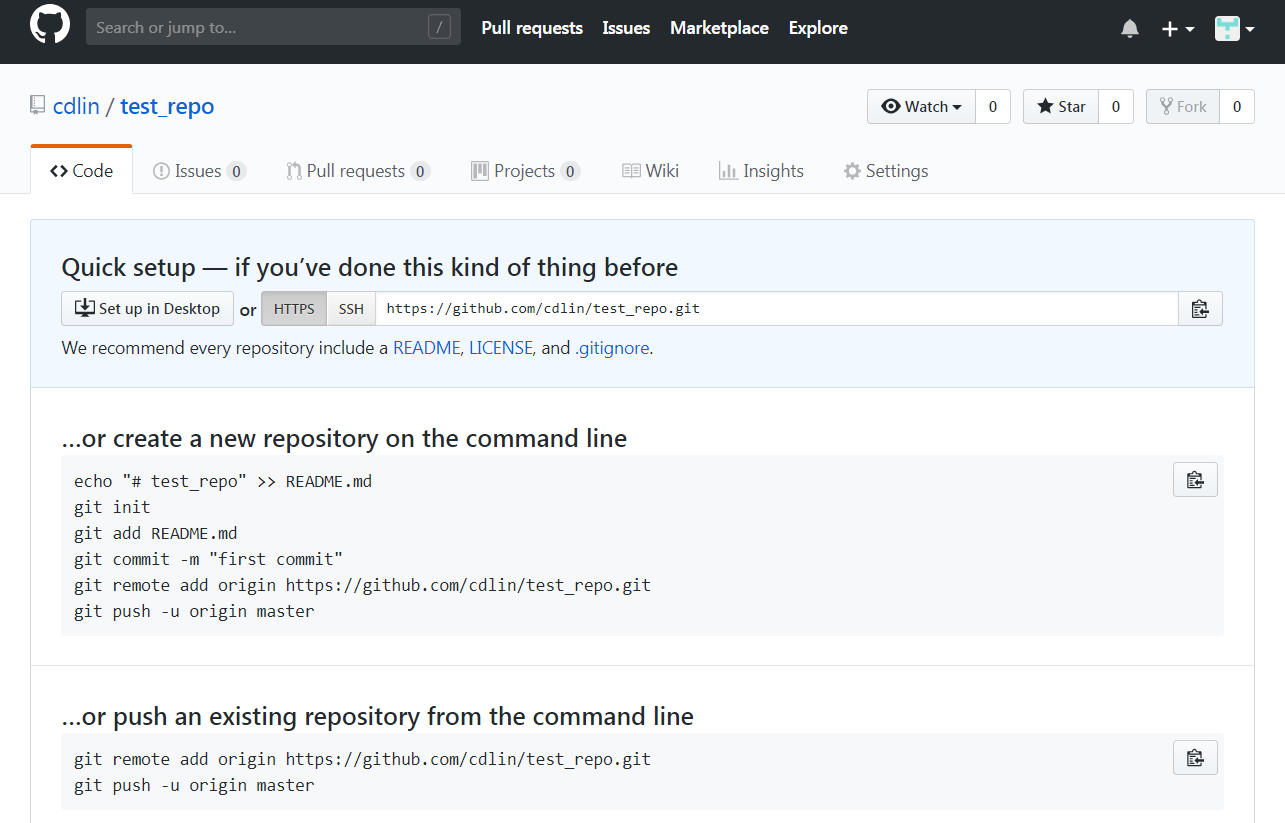
\includegraphics[width=1.0\textwidth]{./auxfiles/github_command.png}
\end{center}
\end{frame}

%%%%%%%%%%%%%%%%%%%%%%%%%%%%%%%%%%%%
\begin{frame}[fragile]{Connecting Local and Online Repositories}
Let's link our local repository with the GitHub repository we created earlier.

Check we're still in the same directory with \emph{pwd}
\begin{lstlisting}
$ pwd 
/c/Users/Daniel/Desktop/myproject
$ git remote add origin https://github.com/cdlin/test_repo.git
\end{lstlisting}
This command tells git to add a remote named \emph{origin} for the repository at \emph{https://github.com/cdlin/test\_repo.git}.\\~\\
We can check that the command worked by typing
\begin{lstlisting}[frame=single]
$ git remote -v
origin  https://github.com/cdlin/test_repo.git (fetch)
origin  https://github.com/cdlin/test_repo.git (push)
\end{lstlisting}
\end{frame}

%%%%%%%%%%%%%%%%%%%%%%%%%%%%%%%%%%%%
\begin{frame}[fragile]{Git Push}
We have linked our remote repository (GitHub) with our local repository. Let's push the commit from our local repository to the GitHub repository with \textcolor{blue}{\emph{git push}}
\begin{lstlisting}
$ git push -u origin master
\end{lstlisting}
It may ask for your GitHub username and password
\begin{lstlisting}[frame=single]
$ git push -u origin master
Enumerating objects: 3, done.
Counting objects: 100% (3/3), done.
Writing objects: 100% (3/3), 234 bytes | 234.00 KiB/s, done.
Total 3 (delta 0), reused 0 (delta 0)
To https://github.com/cdlin/test_repo.git
* [new branch]      master -> master
Branch 'master' set up to track remote branch 'master' from 'origin'.
\end{lstlisting}
Check your GitHub repository, everything we have done in your local repository should be there.
\end{frame}

%%%%%%%%%%%%%%%%%%%%%%%%%%%%%%%%%%%%
\begin{frame}[fragile]{An overview of the Git Cycle}
We should now be able to see the basic structure of how git works. Once a directory is set up as a Git repository using \textcolor{blue}{\emph{git init}}, any change that we make to that directory is noted by git. The workflow is then as follows:
\begin{enumerate}
	\item
	Modify/create new folders and files.
	\item
	Stage these changes ready to commit by using \textcolor{blue}{\emph{git add}}.
	\item
	Commit the changes using \textcolor{blue}{\emph{git commit}} which permanently saves the current version of that repository.
	\item
	Push the commit with \textcolor{blue}{\emph{git push}} to any remote repository
\end{enumerate}
\end{frame}
%%%%%%%%%%%%%%%%%%%%%%%%%%%%%%%%%%%%
\begin{frame}[fragile]{Undoing a ``bad'' commit}

Suppose we have made some unwanted changes to a file and committed it. For example, we didn't want the change we made to the \emph{code.do}.

\begin{lstlisting}
$ git log --oneline
57e91e5 (HEAD -> master, origin/master) New tex file and added line to code.do
887d395 First draft code.do
\end{lstlisting}

We want the version with the id 887d395. Use \textcolor{blue}{\emph{git checkout}}
\begin{lstlisting}
$ git checkout 887d395 code.do
$ cat code.do
This is a test.
\end{lstlisting}


Note that we are not reversing the commit, but making a new one by replacing the code.do with a previous version.

\begin{lstlisting}
$ git commit -m "Retrieved code.do from previous commit"
[master 9a664b0] Retrieved code.do from previous commit
1 file changed, 1 deletion(-)

$ git status
$ git push -u origin master
\end{lstlisting}
You can check your GitHub repository as well.
\end{frame}



%%%%%%%%%%%%%%%%%%%%%%%%%%%%%%%%%%%%
\begin{frame}[fragile]{Hard delete unpublished commits}

Now suppose that we really want to eliminate all traces of a series of particularly bad commits. For example, suppose we have committed the following:
\begin{lstlisting}
$ nano code.do
\end{lstlisting}
Type a random sentence
\begin{lstlisting}
This is a test.
This line will literally erase all my work.
\end{lstlisting}
\begin{lstlisting}
$ git add code.do
$ git commit -m "Updated code"
[master 612ff94] Updated code
1 file changed, 1 insertion(+)
\end{lstlisting}

We can go back to our previous commit with \textcolor{blue}{\emph{git reset}}

\begin{lstlisting}
$ git log --oneline
612ff94 (HEAD -> master) Updated code
9a664b0 (origin/master) Retrieved code.do from previous commit
57e91e5 New tex file and added line to code.do
887d395 First draft code.do

$ git reset --hard 9a664b0
HEAD is now at 9a664b0 Retrieved code.do from previous commit
\end{lstlisting}
\end{frame}

%%%%%%%%%%%%%%%%%%%%%%%%%%%%%%%%%%%%
\begin{frame}[fragile]{Undo published commits with new commits}

Note: you should never use \textcolor{blue}{\emph{git reset}} after the commits you want to undo have been pushed to a public repository. Instead, it is possible to use \textcolor{blue}{\emph{git revert}} to undo one or more target commits.

\begin{lstlisting}
$ git log --oneline
9a664b0 (HEAD -> master, origin/master) Retrieved code.do from previous commit
57e91e5 New tex file and added line to code.do
887d395 First draft code.do

$ git revert 9a664b0
[master deba8ff] Revert "Retrieved code.do from previous commit"
1 file changed, 1 insertion(+)
\end{lstlisting}

This doesn't change the history of the commits and is therefore preferable.\\
\medskip
Note: you can revert multiple commits at the same time; this will in turn create multiple new commits.
See \href{https://github.com/blog/2019-how-to-undo-almost-anything-with-git}{this blog post} about all the differences between undoing commits.
\end{frame}
%%%%%%%%%%%%%%%%%%%%%%%%%%%%%%%%%%%%
\begin{frame}{Git Visualization}
\begin{center}
	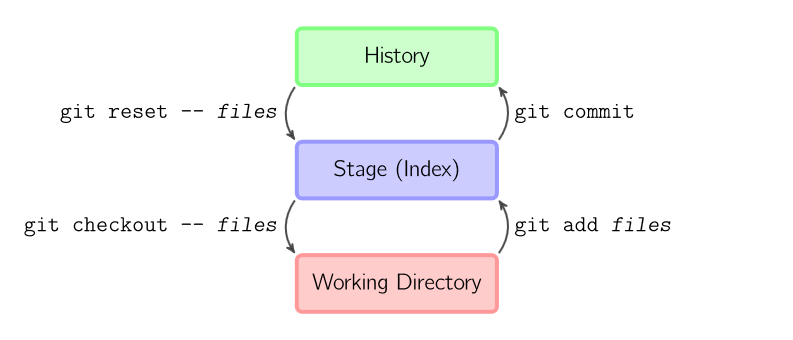
\includegraphics[width=1.0\textwidth]{./auxfiles/basic-usage.png}
\end{center}
\end{frame}



%%%%%%%%%%%%%%%%%%%%%%%%%%%%%%%%%%%%
\begin{frame}[fragile]{Git Pull}
We can download changes from the remote repository (GitHub) to the local one with \textcolor{blue}{\emph{git pull}}:

\begin{lstlisting}
$ git pull origin master
From https://github.com/cdlin/test_repo
* branch            master     -> FETCH_HEAD
Already up to date.
\end{lstlisting}

Pulling has no effect in this case because the two repositories are already synchronized. If someone else had pushed some changes to the repository on GitHub, though, this command would download them to our local repository.\\

\end{frame}

%%%%%%%%%%%%%%%%%%%%%%%%%%%%%%%%%%%%
\begin{frame}[fragile]{Git Clone}
Suppose you start working on a project with an existing GitHub repository. Instead of creating a new repository here with \emph{git init}, we will \textcolor{blue}{\emph{git clone}} the existing repository from GitHub.
\begin{lstlisting}
$cd ../myproject2
$ git clone https://github.com/cdlin/test_repo.git
Cloning into 'test_repo'...
remote: Counting objects: 9, done.
remote: Compressing objects: 100% (5/5), done.
remote: Total 9 (delta 0), reused 9 (delta 0), pack-reused 0
Unpacking objects: 100% (9/9), done.
\end{lstlisting}
We now has two copies of the repository on our Desktop.
\end{frame}

%%%%%%%%%%%%%%%%%%%%%%%%%%%%%%%%%%%%
\begin{frame}[fragile]{Acknowledgment}

This presentation follows the introduction to git by Meghan Nelson on Hubspot. Her tutorial can be found at: \href{https://product.hubspot.com/blog/git-and-github-tutorial-for-beginners}{\color{blue}{https://product.hubspot.com/blog/git-and-github-tutorial-for-beginners}}
\end{frame}

%%%%%%%%%%%%%%%%%%

\end{document}
